\subsection{DC Transfer}

The DC Transfer graph shown in figure \ref{fig:DCtrans} shows the change in the op-amps $V_{out}$ with a voltage input and no feedback.
As expected the output rises fairly suddenly from positive saturation to negative saturation.

\begin{figure}[H]
	\centering
	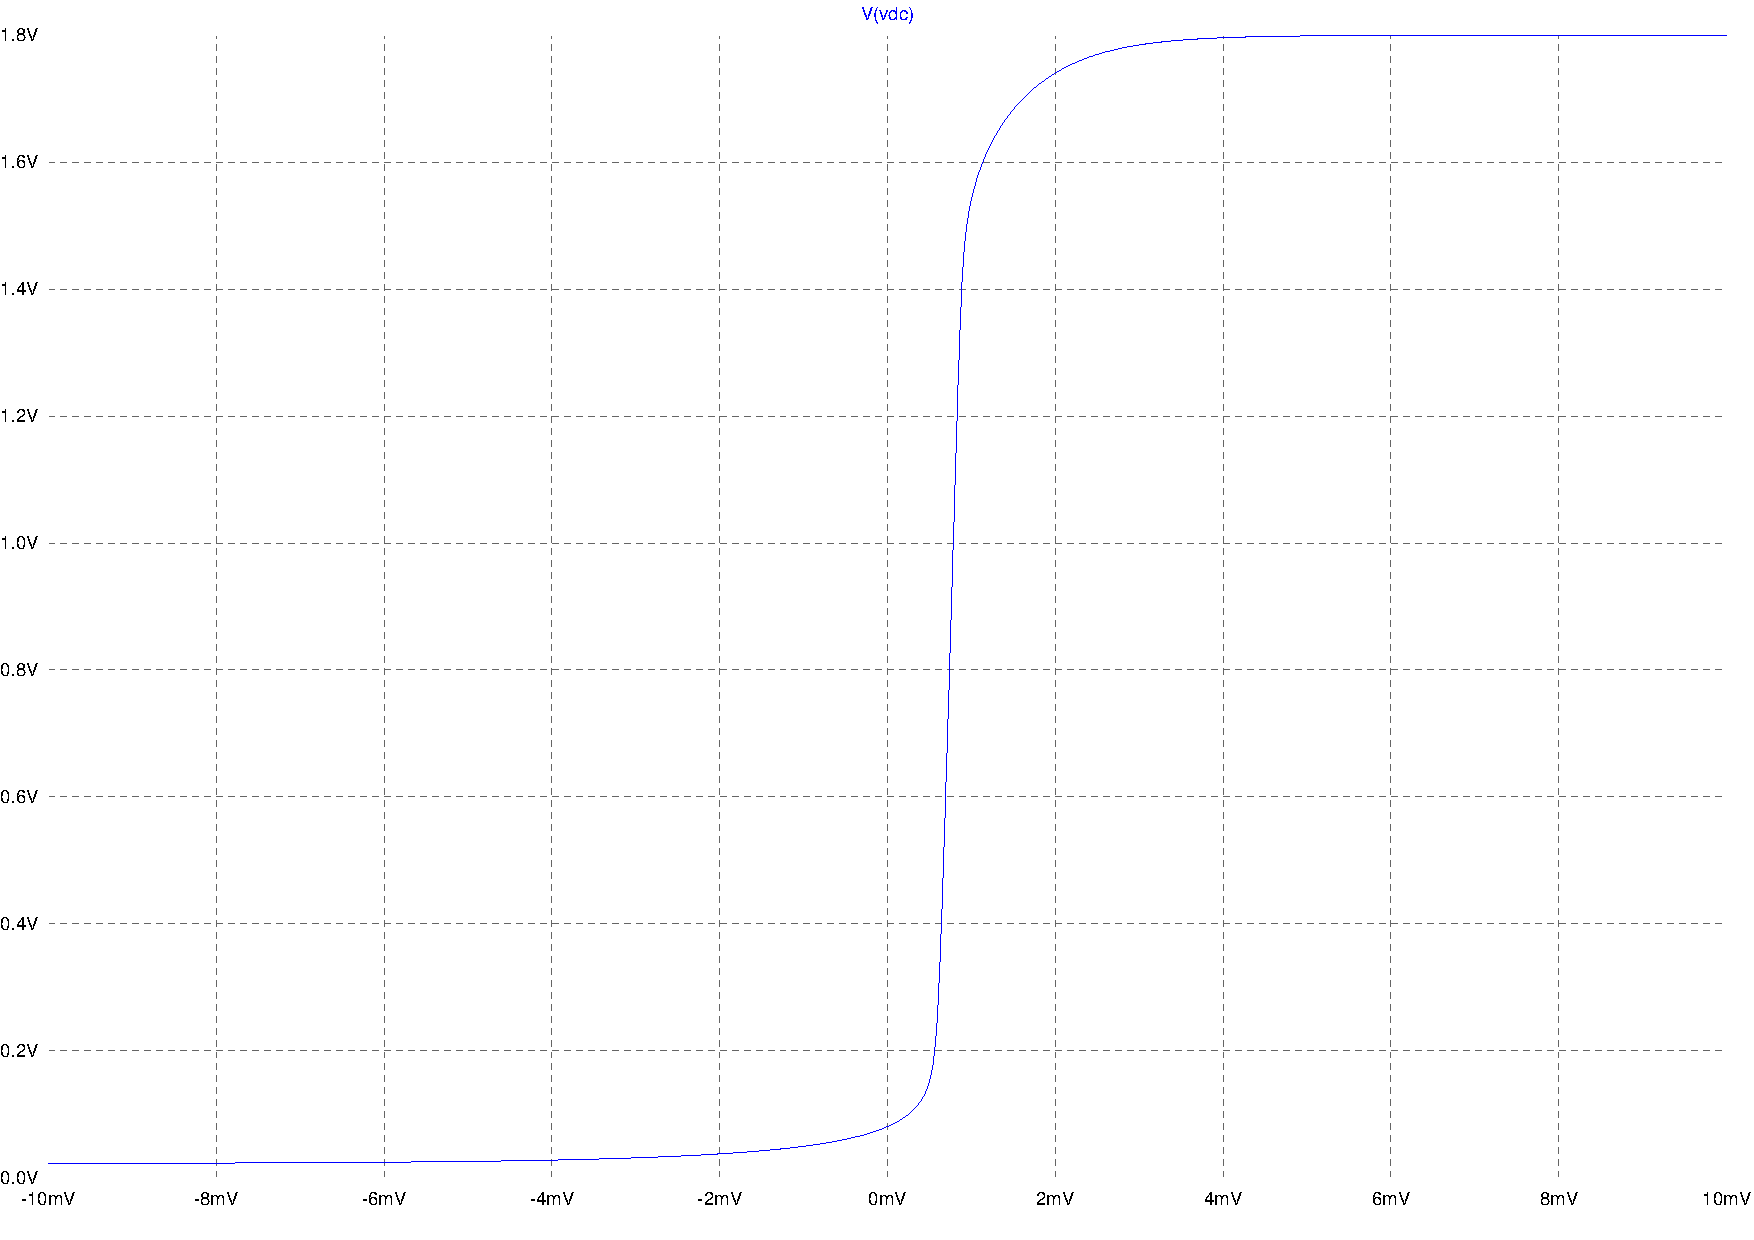
\includegraphics[width=\textwidth]{./images/DCTransfer-out.pdf}
	\caption{$V_{out}$ vs. $V_{in}$ DC transfer}
	\label{fig:DCtrans}
\end{figure}

The linear region can be seen to be extending from $0.2V$ - $1.4V$.
The offset at the centre of this range is $0.8mV$

\begin{figure}[h]
	\centering
	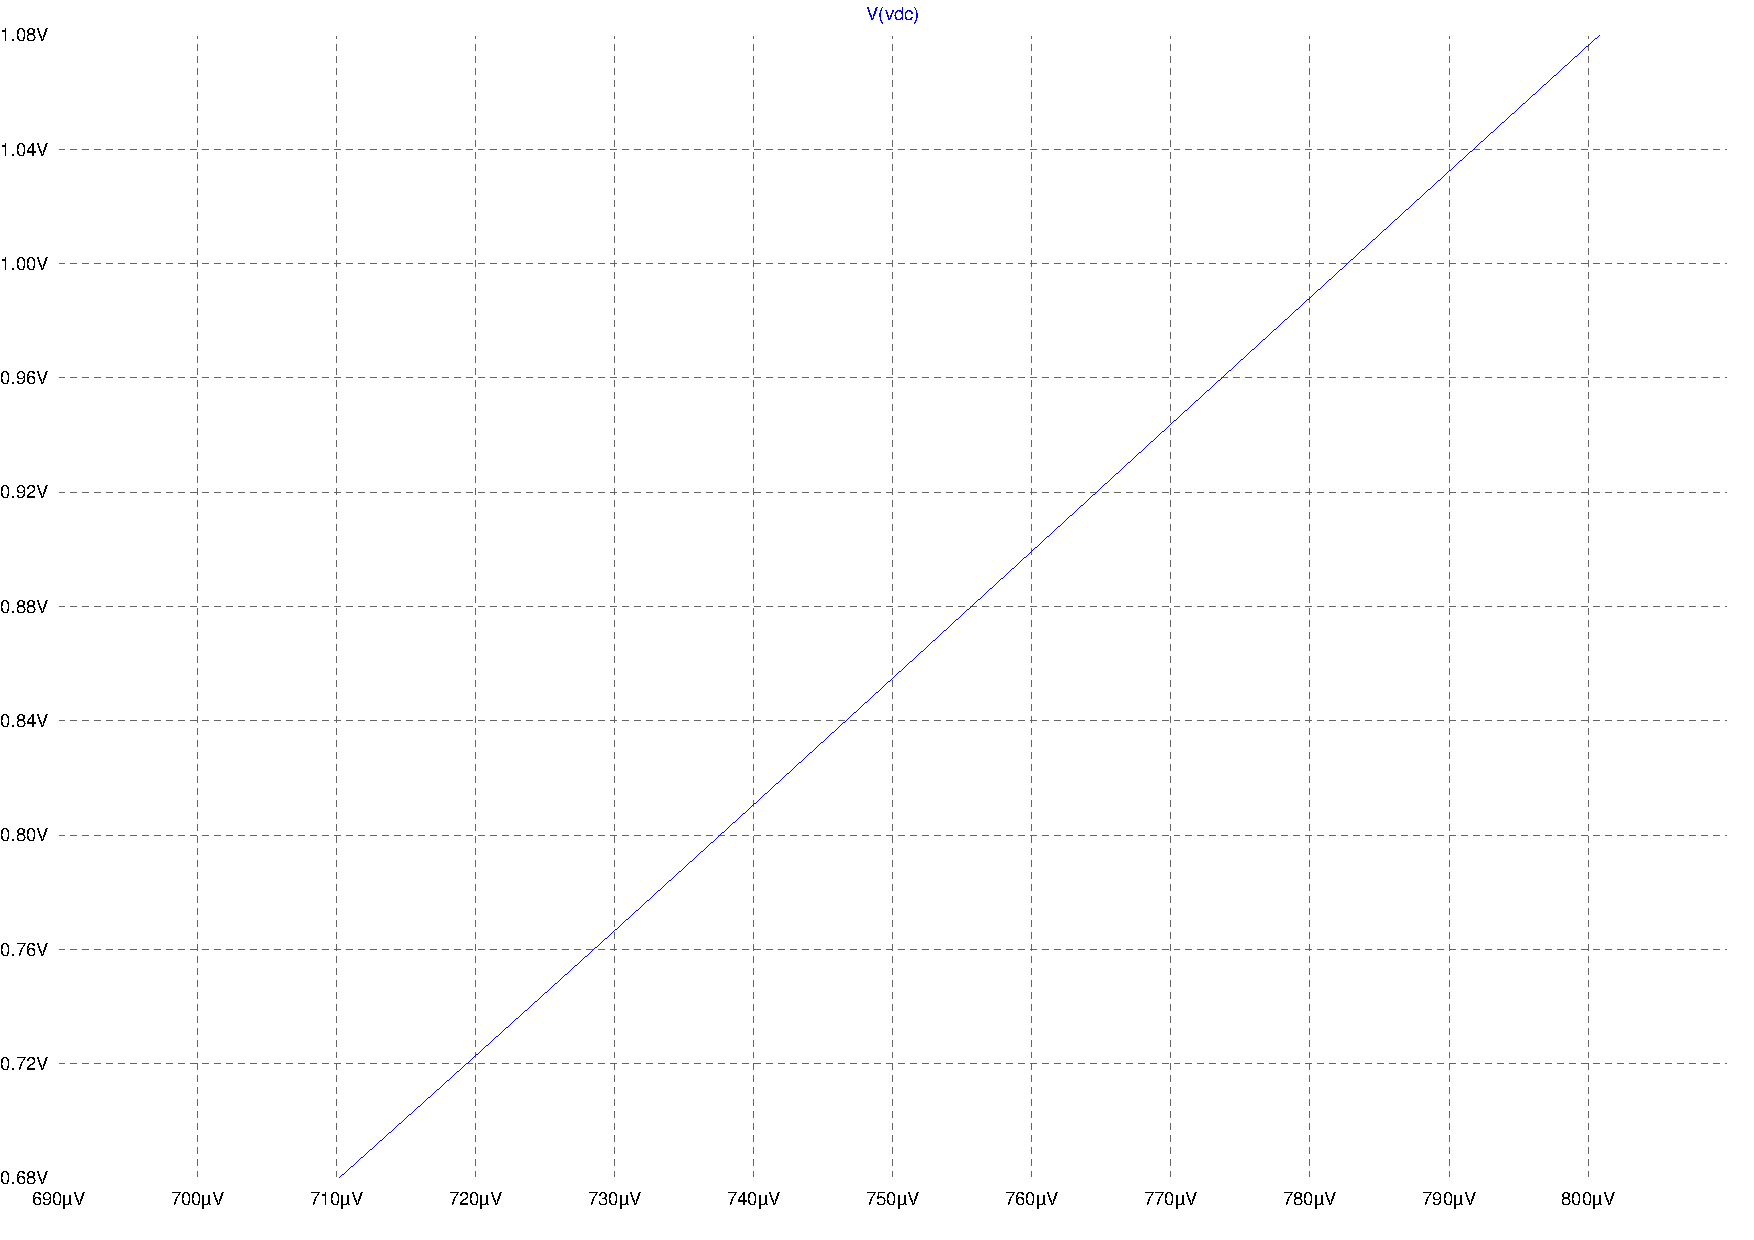
\includegraphics[width=\textwidth]{./images/DCTransfer-zoom.pdf}
	\caption{$V_{out}$ vs. $V_{in}$ DC transfer}
	\label{fig:DCzoom}
\end{figure}

Using this diagram we can determine the gain of the device.
$A_{v} = \frac{\Delta V_{out}}{\Delta V_{in}}$ \\
$A_{v} = \frac{1.00 - 0.8}{\num{783e-6} - \num{737e-6}}$
$A_{v} = 4347.83$
$A_{v} = 72dB$

As the linear region has a gain of $72dB$ between $0.2V$ to $1.4V$ this shows the gain is covering the entire desired output range.
